\section[I BUS]{I BUS}
\label{sec:bus}
\sectionframe{images/covers/cover_bus.jpg}{I BUS}	 


%\subsection[Central Processing Unit]{Central Processing Unit}
%\begin{frame}
%	\frametitle{Central Processing Unit}
%	
%%	\begin{block}{Central Processing Unit}
%		Una CPU, \textbf{central processing unit} (unità centrale di elaborazione o processore centrale), indica un'unità o sottosistema logico e fisico che sovraintende alle \textbf{funzionalità logiche di elaborazione} principali di un computer.
%		La CPU è un'elaborata combinazione di transistor che può essere definita \textit{circuito integrato}.\\~\\
%		\pause
%		All'interno della CPU individuiamo tre elementi fondamentali:
%		\begin{itemize}
%			\item \textbf{la CU}, \textit{Control Unit} (l’unità di controllo):\\
%			coordina l'esecuzione delle operazioni da parte del processore;
%			\item \textbf{la ALU}, \textit{Arithmetic-Logic Unit} (l’Unità Aritmetico-Logica):\\
%			si occupa di eseguire le operazioni aritmetico-logiche;
%			\item \textbf{i registri di memoria}:\\
%			diverse \textit{celle di memoria} dedicate a scopi specifici che vengono utilizzati per il controllo dell'esecuzione di un programma.
%		\end{itemize}
%%	\end{block}
%	
%\end{frame}



\subsection[Lo scopo dei BUS]{Lo scopo dei BUS}


%\begin{frame}
%	\frametitle{Lo scopo dei BUS}
%	
%	\begin{block}{I BUS: le autostrade per i bit}
%		Il BUS nei computer è un sistema di comunicazione che trasmette dati e segnali tra le diverse componenti del sistema, come processori, memoria e dispositivi. Distinguiamo due categorie di BUS:
%		\begin{itemize}
%			\item L'\textbf{internal BUS} (o \textbf{system BUS}): connette componenti all'interno della scheda madre, facilitando lo scambio di dati tra CPU, RAM e altre parti.
%			\item L' \textbf{external BUS}: collega la scheda madre a dispositivi esterni come unità di archiviazione e schede di espansione. 
%		\end{itemize}
%		
%	\end{block}
%	
%\end{frame}

\begin{frame}
	\frametitle{Lo scopo dei BUS}
	
	\begin{block}{}
		I processori operano su $1^i$ e $0^i$. Gli $1^i$ e gli $0^i$ viaggiano da un punto all'altro all'interno del processore, così come all'esterno verso altri chip.
		Per spostare gli $1^i$ e gli $0^i$, vengono utilizzate \textbf{linee elettroniche} chiamate \textbf{BUS}; una sorta di autostrade per i bit. Distinguiamo tra:
		\begin{itemize}
			\item \textbf{internal BUS}: le linee elettroniche \textit{	\underline{interne alla CPU}}. Nell'8086, il BUS dati interno comprende 16 linee separate, ciascuna delle quali contiene un 1 o uno 0. Nei processori odierni si hanno fino a 64/128 linee separate.
			\item \textbf{external BUS}: utilizzato quando la CPU necessita di comunicare con dei \textit{\underline{dispositivi esterni}}, come una stampante. L'external BUS collega il processore agli adattatori, alla tastiera, al mouse, al disco rigido e ad altri dispositivi.
				I processori odierni hanno BUS esterni con 64/128 bit.
		\end{itemize}
		
	\end{block}
	
\end{frame}


\subsection[Internal BUS ed external BUS]{Internal BUS ed external BUS}
\begin{frame}
	\frametitle{Internal BUS ed external BUS}
	  
	\begin{figure}[!htbp]
		\centering
		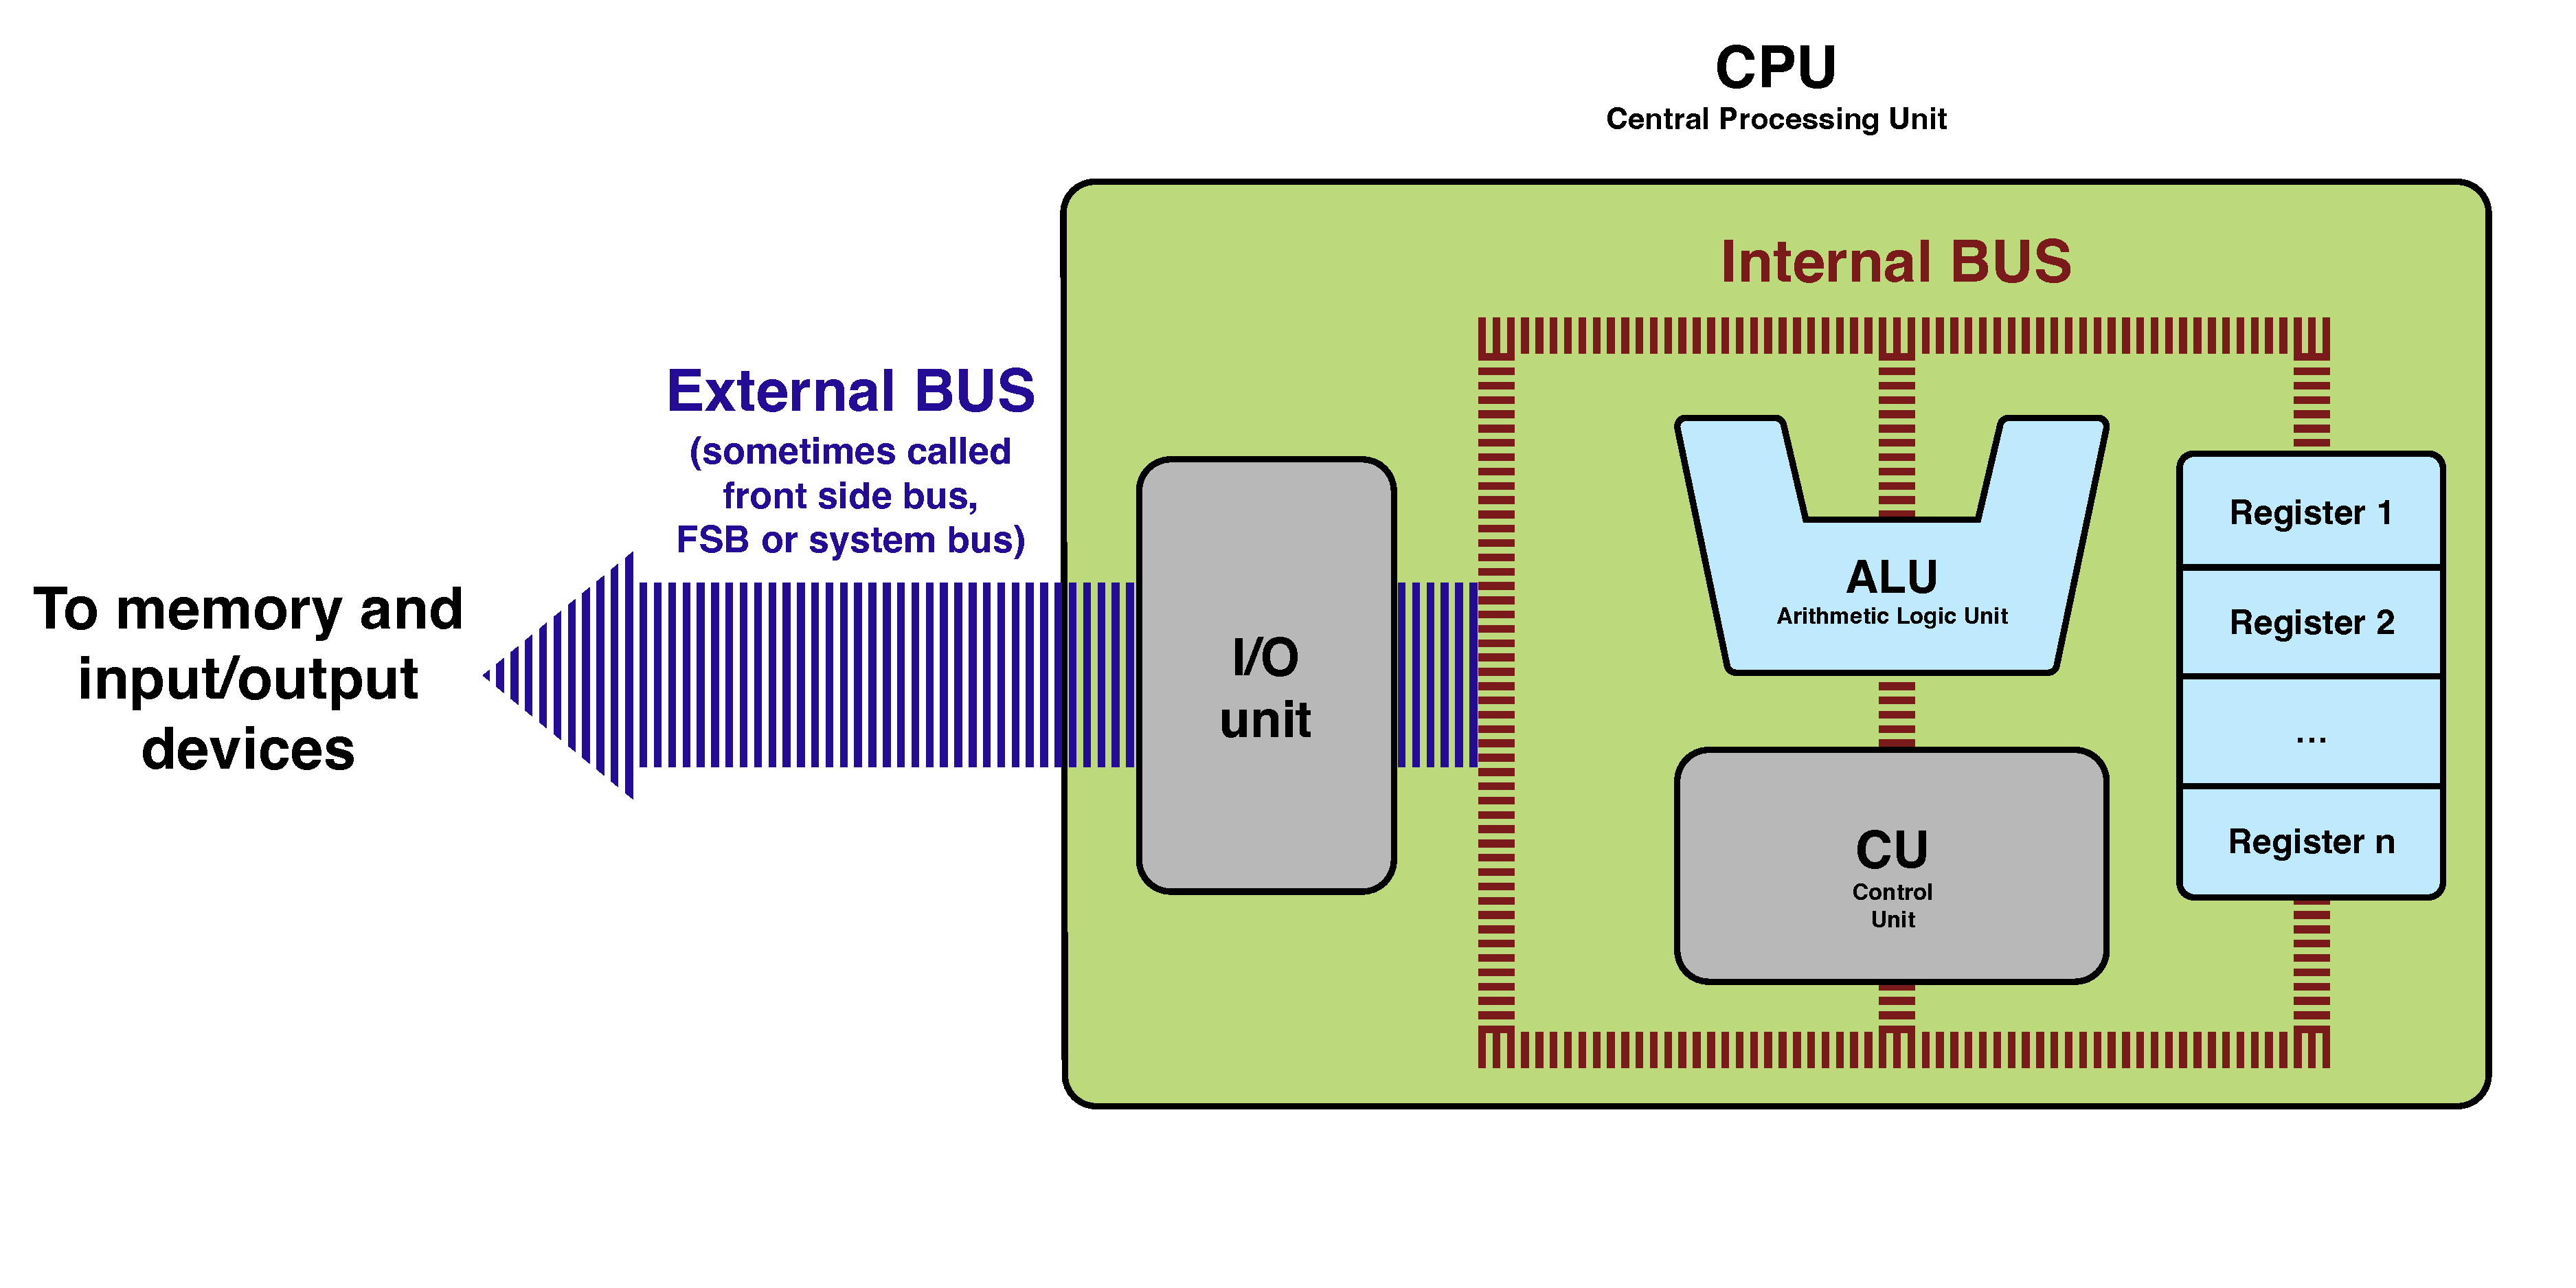
\includegraphics[width=1.0\linewidth]{images/6_bus/bus_internal_external.pdf}
		%\caption{}
%		\label{}
	\end{figure}
\end{frame}



\subsection[Master \& Slave]{Master \& Slave}
\begin{frame}
	\frametitle{Master \& Slave}
	
	\begin{block}{Il master e lo slave}
		Nei sistemi informatici, l'architettura del bus può coinvolgere dispositivi che agiscono come \textit{master} e \textit{slave} durante le operazioni di comunicazione.
		\begin{itemize}
			\item Il \textbf{master} è il dispositivo che inizia e controlla l'operazione di trasferimento dati. Detiene il controllo del flusso di dati e inizia le richieste di lettura o scrittura ad altri dispositivi. Ad esempio, una CPU può essere il master quando richiede dati dalla memoria RAM.
			\item Lo \textbf{slave}, d'altro canto, risponde alle richieste del master e fornisce i dati richiesti o accetta i dati da scrivere. Un esempio tipico è un dispositivo di archiviazione come un'unità SSD o un'unità disco rigido, che risponde alle richieste di lettura o scrittura provenienti dalla CPU (master).
		\end{itemize}
		
	\end{block}
	
\end{frame}


% https://www.tablesgenerator.com/#
\begin{frame}
	\frametitle{Master \& Slave}
	
	\begin{block}{}
		Questo concetto è fondamentale per garantire che le comunicazioni avvengano in modo coordinato e senza conflitti, consentendo al sistema di funzionare in modo efficiente e affidabile.
		\begin{table}[]
			\begin{tabular}{|c|c|c|}
			\hline
			\rowcolor[HTML]{ffce93} 
			\textbf{Master} & \textbf{Slave}     & \textbf{Situazione}                                      \\ \hline
			\rowcolor[HTML]{EFEFEF} 
			CPU             & Memoria            & \shortstack{Fetch dell'istruzione\\  o degli operandi}                   \\ \hline
			\rowcolor[HTML]{EFEFEF} 
			CPU             & Dispositivo di I/O & \shortstack{Operazione di lettura \\o scrittura con dispositivo di I/O} \\ \hline
			\rowcolor[HTML]{EFEFEF} 
			CPU             & Memoria            & \shortstack{Operazione di lettura \\o scrittura su memoria}             \\ \hline
			\rowcolor[HTML]{EFEFEF} 
			I/O             & Memoria            & \shortstack{DMA \\(Direct Memory Access)}                               \\ \hline
			\end{tabular}
		\end{table}
		
	\end{block}
	
\end{frame}


\subsection[Aumentare le prestazioni dei BUS]{Aumentare le prestazioni dei BUS}
\begin{frame}
	\frametitle{Aumentare le prestazioni dei BUS}
	  
	\begin{block}{}
		Per migliorare le prestazioni di un BUS, vengono utilizzate diverse tecniche di progettazione e ottimizzazione. Alcune di queste includono:
		\begin{itemize}
			\item \textbf{Aumento della larghezza del bus}: incrementare il numero di linee dei bus consente di trasferire più dati contemporaneamente, accelerando il trasferimento di informazioni tra i dispositivi collegati.
			\item \textbf{Aumento della velocità di clock}: aumentare la frequenza di clock del bus consente di aumentare la velocità di trasferimento dei dati. Tuttavia, ciò può portare a problemi di interferenza elettronica e consumo energetico più elevato.
			\item \textbf{Caching}: l'utilizzo di cache può ridurre la necessità di trasferimenti frequenti tra la CPU e la memoria principale. Le cache sono memorie veloci e di piccole dimensioni che conservano copie dei dati più utilizzati dalla CPU.
		\end{itemize}
		
	\end{block}

\end{frame}


\begin{frame}
	\frametitle{Aumentare le prestazioni dei BUS: larghezza del BUS}
	  
	\begin{figure}[!htbp]
		\centering
		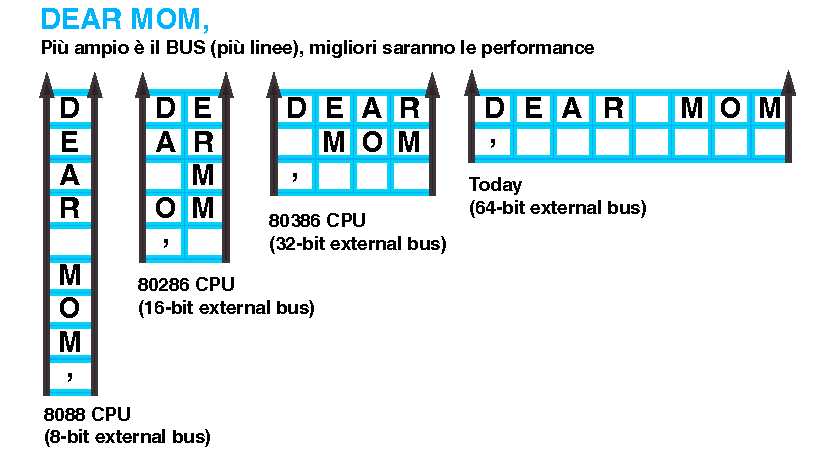
\includegraphics[width=0.715\linewidth]{images/6_bus/bus_size.pdf}
		\caption{per il computer, ogni lettera dell'alfabeto è una diversa combinazione di otto 1 e 0 (in una codifica ASCII ad esempio). Ad esempio, la lettera D è 01000100 e la lettera E è 01000101. La figura dimostra che \underline{aumentando} la \textbf{larghezza del BUS} \underline{aumentano} notevolmente \textbf{le prestazioni} di un computer, in modo simile a come l'aumento del numero di corsie di un'autostrada ne riduce la congestione.}
%		\label{}
	\end{figure}
\end{frame}



\subsection[Valutare le prestazioni dei BUS]{Valutare le prestazioni dei BUS}
\begin{frame}
	\frametitle{Valutare le prestazioni di un BUS}
	  
	\begin{block}{Parametri delle prestazioni di un BUS}
		\begin{itemize}
			\item \textbf{Larghezza}: indica il numero di linee dati di un BUS. Più linee significano maggiore capacità di trasferimento simultaneo di dati.
			\item \textbf{Bit Rate}: è il numero di bit trasmessi o ricevuti in un'unità di tempo, misurato in bit al secondo (bps).
			\item \textbf{Banda}: è la quantità di dati che può essere trasmessa attraverso il bus in un dato intervallo di tempo, espressa solitamente in byte al secondo (Bps).
			\item \textbf{Velocità}: rappresenta la frequenza di clock del BUS per un BUS sincrono, determinando quante volte i dati possono essere trasmessi o ricevuti in un secondo.
		\end{itemize}
		
	\end{block}

\end{frame}


\subsection[BUS sincrono e asincrono]{BUS sincrono e asincrono}
\begin{frame}
	\frametitle{BUS sincrono e asincrono}
	  
	\begin{block}{Parametri delle prestazioni di un BUS}
		I BUS sincroni e asincroni differiscono nel modo in cui gestiscono il timing delle comunicazioni:
		\begin{itemize}
			\item In un \textbf{BUS sincrono}, i dispositivi seguono un orologio comune, coordinando trasmissioni e ricezioni in base a impulsi temporizzati.
				I BUS sincroni offrono maggiore precisione e velocità ma richiedono un'accurata sincronizzazione. 
			\item Nei \textbf{BUS asincroni}, invece, i dati vengono trasmessi senza un clock centralizzato, utilizzando segnali di controllo per indicare l'inizio e la fine dei dati. I BUS asincroni sono più flessibili e tolleranti ma possono essere meno efficienti in termini di velocità di trasferimento.
		\end{itemize}
		
	\end{block}

\end{frame}

% TODO aggiungere esercizi sul BUS sincrono e asincrono
\begin{frame}
	\frametitle{Esercizi sui BUS sincroni}
	
	\begin{block}{Esercizio 1}
		Un bus sincrono presenta le seguenti caratteristiche:
		\begin{scriptsize}
		\begin{enumerate}
			\item durata di un ciclo di clock 25 ns
			\item durata di una trasmissione sul bus 2 cicli di clock
			\item dimensione del bus dati 32 bit
			\item dimensione del bus indirizzi 32 bit
		\end{enumerate}
		\end{scriptsize}
		Qual è il tempo di trasferimento durante un’operazione di lettura (READ) di un dato dalla memoria, sapendo che la memoria principale ha un tempo di ciclo pari a 100 ns e che ciascuna locazione di memoria ha capacità pari a 64 bit?
		
		\begin{scriptsize}
		\begin{itemize}
			\item A. $5 s$
			\item B. $250 ns$
			\item C. $5 \cdot 10^{-7} s$
			\item D. $2 \cdot 10^{-7} s$
		\end{itemize}
		\end{scriptsize}
	
	\end{block}
\end{frame}


\begin{frame}
	\frametitle{Esercizi sui BUS sincroni}
	
	\begin{block}{Esercizio 1: soluzione}
		\begin{figure}[!htbp]
			\centering
			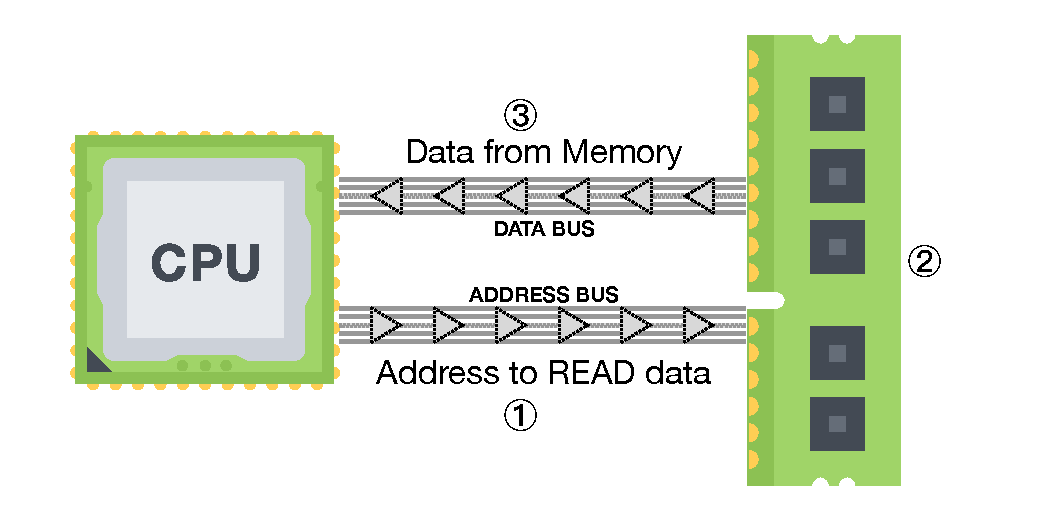
\includegraphics[width=0.86\linewidth]{images/6_bus/bus_synch.pdf}
			\caption{{\color{CpuGreen}1. Invio indirizzo}, {\color{CpuBlue}2. Estrazione del dato}, {\color{CpuRed}3. Invio del dato}}
%			\label{}
		\end{figure}
	\end{block}
\end{frame}


\begin{frame}
	\frametitle{Esercizi sui BUS sincroni}
	
	\begin{block}{Esercizio 1: soluzione}
		Per calcolare il tempo di una lettura è necessario scomporre l'operazione di lettura in tre parti e calcolare la durata di ogni operazione in questo specifico caso:
		\begin{enumerate}
			\item {\color{CpuGreen}Inviare l'indirizzo della locazione di memoria tramite il BUS degli indirizzi: $2\mathrm{T}$}
			\item {\color{CpuBlue}Lettura della parola dalla memoria: $\Big\lceil \frac{100}{25} \Big\rceil \mathrm{T} \rightarrow 4\mathrm{T}$}
			\item {\color{CpuRed} Inviare il dato tramite il BUS dati; ricordando che il BUS dati è ampio 32 bit, mentre il dato da inviare è di 64 bit, sono necessari due invii attraverso il BUS dati, di conseguenza: $2 \cdot 2\mathrm{T} \rightarrow 4\mathrm{T}$}
		\end{enumerate}
		Quindi il tempo di trasferimento per un READ per questa architettura è dato da:
		$$t = {\color{CpuGreen}2\mathrm{T}} + {\color{CpuBlue}4\mathrm{T}} + {\color{CpuRed}4\mathrm{T}} = 10\mathrm{T} = 10 \cdot 25ns = 250ns$$
	\end{block}
\end{frame}


\begin{frame}
	\frametitle{Esercizi sui BUS sincroni}
		
	\begin{block}{Esercizio 2}
		Un bus sincrono presenta le seguenti caratteristiche:
		\begin{scriptsize}
		\begin{enumerate}
			\item durata di un ciclo di clock 15 ns
			\item durata di una trasmissione sul bus 2 cicli di clock
			\item dimensione del bus dati 32 bit
			\item dimensione del bus indirizzi 32 bit
		\end{enumerate}
		\end{scriptsize}
		
		Qual è la velocità di trasferimento durante un’operazione di lettura (READ) di un dato dalla memoria, sapendo che la memoria principale ha un tempo di ciclo pari a 100 ns e che ciascuna locazione di memoria ha capacità pari a 64 bit?
		
		\begin{scriptsize}
		\begin{itemize}
			\item A. $64 bit/195 ns$
			\item B. $32 bit/195 ns$
			\item C. $32 bit/(195 \cdot 10^{-9})$
			\item D. $4 byte/(195 \cdot 10^{-9})$
		\end{itemize}
		\end{scriptsize}
	
	\end{block}
\end{frame}


\begin{frame}
	\frametitle{Esercizi sui BUS sincroni}
	
	\begin{block}{Esercizio 2: soluzione}
		\begin{figure}[!htbp]
			\centering
			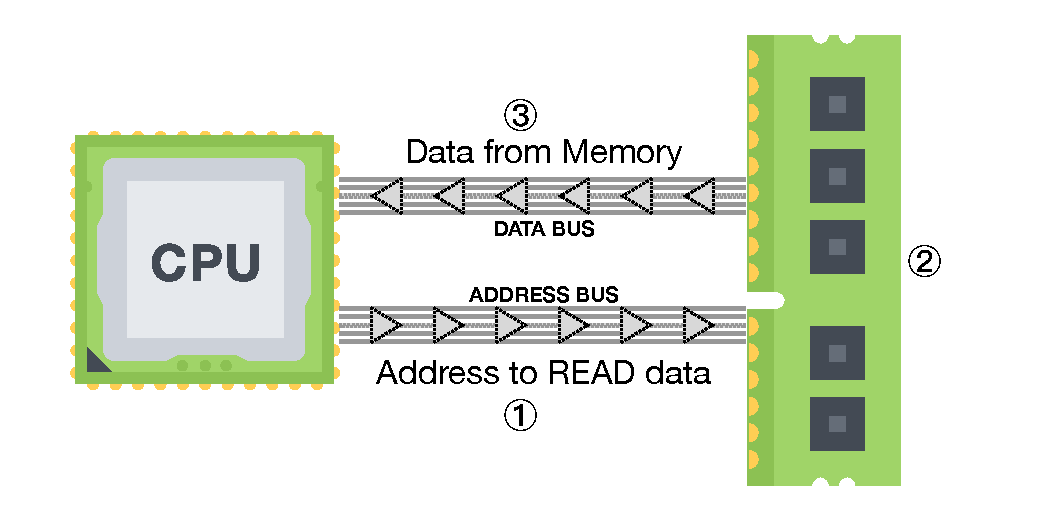
\includegraphics[width=0.86\linewidth]{images/6_bus/bus_synch.pdf}
			\caption{{\color{CpuGreen}1. Invio indirizzo}, {\color{CpuBlue}2. Estrazione del dato}, {\color{CpuRed}3. Invio del dato}}
%			\label{}
		\end{figure}
	\end{block}
\end{frame}


\begin{frame}
	\frametitle{Esercizi sui BUS sincroni}
	
	\begin{block}{Esercizio 2: soluzione}
		Per calcolare la velocità di trasferimento in lettura è necessario scomporre l'operazione di lettura in tre parti e calcolare la durata di ogni operazione in questo specifico caso:
		\begin{enumerate}
			\item {\color{CpuGreen}Inviare l'indirizzo della locazione di memoria tramite il BUS degli indirizzi: $2\mathrm{T}$}
			\item {\color{CpuBlue}Lettura della parola dalla memoria: $\Big\lceil \frac{100}{15} \Big\rceil \mathrm{T} \rightarrow 7\mathrm{T}$}
			\item {\color{CpuRed} Inviare il dato tramite il BUS dati; ricordando che il BUS dati è ampio 32 bit, mentre il dato da inviare è di 64 bit, sono necessari due invii attraverso il BUS dati, di conseguenza: $2 \cdot 2\mathrm{T} \rightarrow 4\mathrm{T}$}
		\end{enumerate}
		Quindi calcoliamo la velocità di lettura per questa architettura come:
		$$t = {\color{CpuGreen}2\mathrm{T}} + {\color{CpuBlue}7\mathrm{T}} + {\color{CpuRed}4\mathrm{T}} = 13\mathrm{T} = 13 \cdot 15ns = 195ns \rightarrow 64bit/195ns$$
	\end{block}
\end{frame}


\begin{frame}
	\frametitle{Esercizi sui BUS sincroni}
	
	\begin{block}{Esercizio 2: soluzione}
		Non è richiesto dall'esercizio ma qualora volessimo calcolare la velocità di trasferimento in termini di byte/s ripartiamo dal risultato di $64bit/195ns$ e procediamo a calcolare la velocità come segue:\\~\\
		
		\begin{scriptsize}
		$$\frac{64bit}{195ns} = \frac{8byte}{195 \cdot 10^{-9} s} = \frac{{\color{CpuBlue}8} \cdot 10^{9}byte}{{\color{CpuBlue}195}s}= {\color{CpuBlue}0.041} \cdot 10^{9} byte/s = 410 \cdot 10^{6} byte/s \simeq 410 MB/s$$
		\end{scriptsize}
		
	\end{block}
\end{frame}



\begin{frame}
	\frametitle{Esercizi sui BUS sincroni}
		
	\begin{block}{Esercizio 3}
		Un bus sincrono presenta le seguenti caratteristiche:
		\begin{scriptsize}
		\begin{enumerate}
			\item linea dati di 32 bit
			\item durata di un ciclo di clock 50 ns
			\item il tempo di trasmissione su bus è 1 ciclo di clock
			\item il tempo per leggere una parola dalla memoria è 200 ns
		\end{enumerate}
		\end{scriptsize}
		
		Qual è la banda massima di trasmissione per la lettura di una parola dalla memoria da un altro dispositivo?
		
		\begin{scriptsize}
		\begin{itemize}
			\item A. $15MB/s$
			\item B. $2MB/s$
			\item C. $20MB/s$
			\item D. $13.3MB/s$
		\end{itemize}
		\end{scriptsize}
	
	\end{block}
\end{frame}


\begin{frame}
	\frametitle{Esercizi sui BUS sincroni}
	
	\begin{block}{Esercizio 3: soluzione}
		\begin{figure}[!htbp]
			\centering
			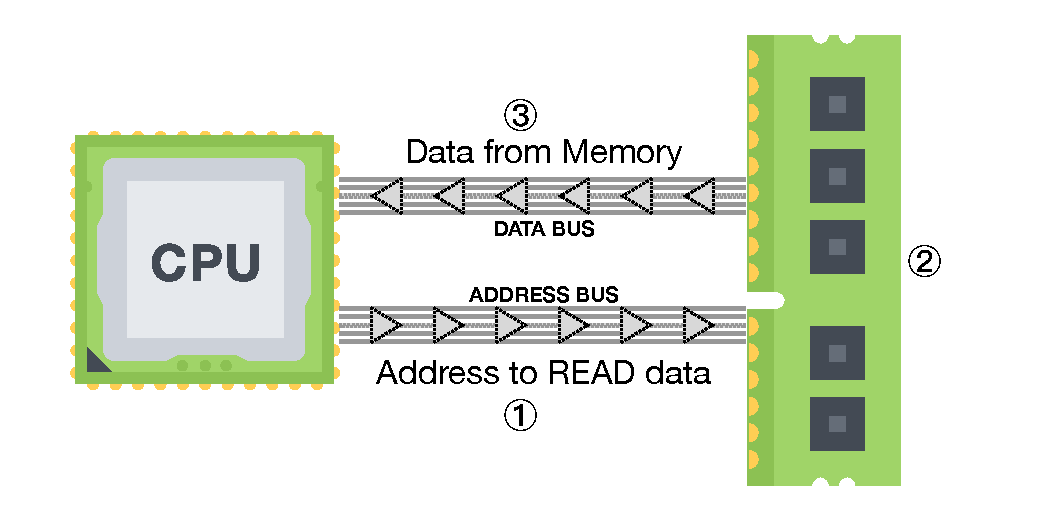
\includegraphics[width=0.86\linewidth]{images/6_bus/bus_synch.pdf}
			\caption{{\color{CpuGreen}1. Invio indirizzo}, {\color{CpuBlue}2. Estrazione del dato}, {\color{CpuRed}3. Invio del dato}}
%			\label{}
		\end{figure}
	\end{block}
\end{frame}


\begin{frame}
	\frametitle{Esercizi sui BUS sincroni}
	
	\begin{block}{Esercizio 3: soluzione}
		Per calcolare la banda di trasmissione per la lettura è necessario scomporre l'operazione di lettura in tre parti e calcolare la durata di ogni operazione in questo specifico caso:
		\begin{enumerate}
			\item {\color{CpuGreen}Inviare l'indirizzo della locazione di memoria tramite il BUS degli indirizzi: $1\mathrm{T}$}
			\item {\color{CpuBlue}Lettura della parola dalla memoria: $\Big\lceil \frac{200}{50} \Big\rceil \mathrm{T} \rightarrow 4\mathrm{T}$}
			\item {\color{CpuRed} Inviare il dato tramite il BUS dati; ricordando che il BUS dati è ampio 32 bit e il dato da inviare è di 32 bit, è sufficiente un invio attraverso il BUS dati, di conseguenza: $1\mathrm{T}$}
		\end{enumerate}
		Quindi calcoliamo la velocità di lettura per questa architettura come:
		$$t = {\color{CpuGreen}1\mathrm{T}} + {\color{CpuBlue}4\mathrm{T}} + {\color{CpuRed}1\mathrm{T}} = 6\mathrm{T} = 6 \cdot 50ns = 300ns \rightarrow 32bit/300ns = 4byte/300ns$$
	\end{block}
\end{frame}


\begin{frame}
	\frametitle{Esercizi sui BUS sincroni}
	
	\begin{block}{Esercizio 3: soluzione}
		Possiamo quindi calcolare la banda massima di trasmissione per la lettura in termini di byte/s ripartendo dal risultato di $4byte/300ns$:\\~\\
		
		\begin{scriptsize}
		$$\frac{4byte}{300ns} = \frac{4byte}{300 \cdot 10^{-9} s} = \frac{{\color{CpuBlue}4} \cdot 10^{9}byte}{{\color{CpuBlue}300}s}= {\color{CpuBlue}0.01333} \cdot 10^{9} byte/s = 13.33 \cdot 10^{6} byte/s \simeq 13.33 MB/s$$
		\end{scriptsize}
		
	\end{block}
\end{frame}


%\begin{frame}
%
%			\begin{itemize}
%				\item \textbf{Hit rate} di 82\% \hspace{9.5em} $\rightarrow$ \hspace{2em} ${\color{CpuGreen}h} = 0.8$
%				\item \textbf{Hit time} di 2ns \hspace{9.7em} $\rightarrow$ \hspace{2em} ${\color{CpuBlue}t_c} = 2ns$
%				\item \textbf{Miss penalty} di 500ns \hspace{6.8em} $\rightarrow$ \hspace{2em} ${\color{CpuPink}t_p} = 500ns$
%			\end{itemize}
%		\end{block}
%		\pause
%		$$t = {\color{CpuGreen}h} \cdot {\color{CpuBlue}t_c} + {\color{CpuRed}m} \cdot {\color{CpuPink}t_p}$$
%		\pause
%		Da cui, sostituendo i valori numerici:
%		\pause
%		$$\qquad \qquad t = {\color{CpuGreen}0.8} \cdot {\color{CpuBlue}2} + {\color{CpuRed}0.2} \cdot {\color{CpuPink}500} = 101.6ns \quad \pause (\ll 500ns)$$
%	
%\end{frame}


%\begin{frame}
%	\frametitle{Il tempo medio di accesso alla cache}
%	
%	\begin{block}{Il tempo medio di accesso alla cache $t$}
%	Possiamo calcolare il \textbf{tempo medio di accesso alla cache} $t$ come segue:\vspace{0.25em} \pause
%		\begin{Large}
%		$$t = {\color{CpuGreen}h} \cdot {\color{CpuBlue}t_c} + {\color{CpuRed}m} \cdot {\color{CpuPink}t_p}$$
%		\end{Large}
%		~\vspace{0.5em} \pause
%		Ovvero si calcola come: \pause
%		\begin{enumerate}
%			\item l'{\color{CpuGreen}\textbf{hit rate}} (prob. di hit) per il {\color{CpuBlue}\textbf{tempo di accesso alla memoria cache}} \pause
%			\item più il \pause
%			\item il {\color{CpuRed}\textbf{miss rate}} (prob. di miss = prob. di non hit) moltiplicato per il {\color{CpuPink}\textbf{tempo necessario ad ottenere il dato dalle memorie "inferiori"}} \pause
%		\end{enumerate}
%		
%		Si noti che è una sorta di media pesata dove i pesi sono dati da $h$ e $m$, ovvero hit rate e miss rate che sono due probabilità tali che ${\color{CpuGreen}h} + {\color{CpuRed}m} = 1$.
%	\end{block}
%	
%\end{frame}





\subsection[L'arbitraggio di un BUS]{L'arbitraggio di un BUS}
\begin{frame}
	\frametitle{L'arbitraggio di un BUS}
	  
	\begin{block}{L'arbitraggio di un BUS}
		L'\textbf{arbitraggio di un BUS} è un processo essenziale nell'architettura dei computer, dove più dispositivi o processori condividono lo stesso BUS per accedere alle risorse di sistema, come memoria o periferiche.\\~\\
		
		L'arbitraggio \underline{gestisce il conflitto di accesso simultaneo dei dispositivi}, \underline{evitando collisioni} e \underline{garantendo l'ordine corretto di accesso}.\\~\\

		Il sistema di arbitraggio \textbf{determina quale dispositivo ha il diritto di utilizzare il bus in un dato momento}, assegnando priorità o utilizzando algoritmi di turni. Ciò evita situazioni di contenzione, in cui più dispositivi cercano di accedere al BUS contemporaneamente, garantendo l'equità e l'efficienza nell'utilizzo delle risorse di sistema.
		
	\end{block}
\end{frame}


\begin{frame}
	\frametitle{L'arbitraggio di un BUS}
	  
	\begin{block}{L'arbitraggio di un BUS}
		Approfondiamo tre tipologie di arbitraggio:
		\begin{enumerate}
			\item arbitraggio centralizzato (daisy chaining a un livello)
			\item arbitraggio centralizzato (daisy chaining con più livelli di priorità)
			\item arbitraggio distribuito.
		\end{enumerate}
		~\\
		Nell'arbitraggio centralizzato il bus viene concesso da un circuito integrato nella CPU chiamato appunto arbitro, invece nell'arbitraggio decentralizzato non esiste questo chip, la concessione del bus viene gestita dagli stessi dispositivi.

	\end{block}
\end{frame}



\subsubsection[Daisy chaining a un livello]{Daisy chaining a un livello}
\begin{frame}
	\frametitle{Daisy chaining a un livello}
	  
	\begin{block}{Daisy chaining a un livello}
		\begin{figure}[!htbp]
			\centering
			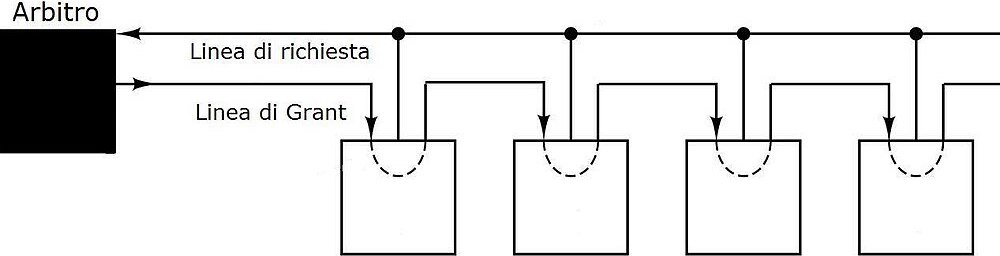
\includegraphics[width=0.8\linewidth]{images/6_bus/daisy_chaining_lev_1.jpg}
%			\caption{}
%			\label{}
		\end{figure}
	\end{block}
\end{frame}


\subsubsection[Daisy chaining con più livelli di priorità]{Daisy chaining con più livelli di priorità}
\begin{frame}
	\frametitle{Daisy chaining con più livelli di priorità}
	  
	\begin{block}{Daisy chaining con più livelli di priorità}
		\begin{figure}[!htbp]
			\centering
			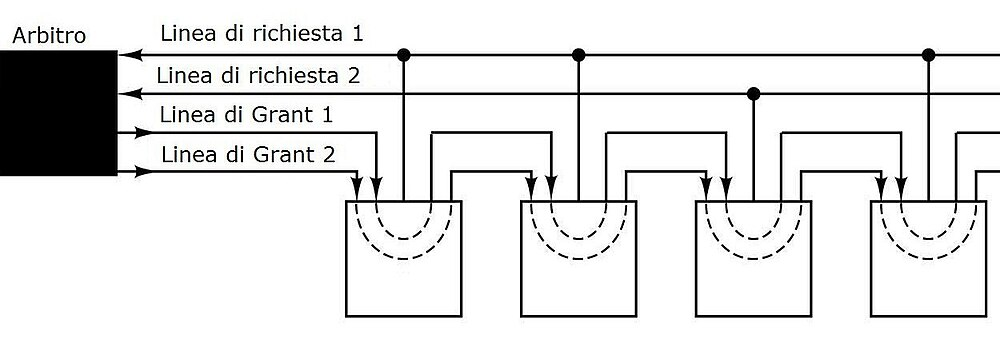
\includegraphics[width=0.8\linewidth]{images/6_bus/daisy_chaining_lev_n.jpg}
%			\caption{}
%			\label{}
		\end{figure}
	\end{block}
\end{frame}



\subsubsection[Arbitraggio distribuito]{Arbitraggio distribuito}
\begin{frame}
	\frametitle{Arbitraggio distribuito}
	  
	\begin{block}{Arbitraggio distribuito}
		\begin{figure}[!htbp]
			\centering
			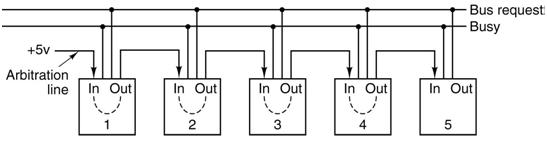
\includegraphics[width=0.8\linewidth]{images/6_bus/daisy_chaining_distributed.jpg}
%			\caption{}
%			\label{}
		\end{figure}
		
	\end{block}
\end{frame}








